\documentclass[a4paper,10pt]{article}
\usepackage[utf8]{inputenc}
\usepackage{geometry} 	%pour les marges
\usepackage{color} %pour la definition de nouvelles couleurs
\usepackage{graphicx} %pour ajouter des images 
\usepackage[final]{pdfpages} 
\usepackage[francais]{babel} % ``Franciser '' le document
\usepackage{lscape}
\usepackage	
  [colorlinks=false, urlcolor=red, breaklinks, pagebackref, citebordercolor={0 0 0}, 
  filebordercolor={0 0 0}, linkbordercolor={0 0 0}, pagebordercolor={0 0 0}, 
  runbordercolor={0 0 0}, urlbordercolor={0 0 0}, pdfborder={0 0 0}]
	{hyperref} % Ajouter le package des lien redirigeant sans les encadrer 
\usepackage{eurosym}
\usepackage{dirtree}
\usepackage{comment}

%couleurs pour les morceaux de code
\definecolor{codegreen}{rgb}{0,0.6,0}
\definecolor{codered}{rgb}{1,0.1,0.2}
\definecolor{codegray}{rgb}{0.5,0.5,0.5}
\definecolor{codepurple}{rgb}{0.58,0,0.82}
\definecolor{backcolour}{rgb}{0.95,0.95,0.92}
 

%modificaion des marges
\geometry{hmargin=2.5cm,vmargin=3cm}


%opening
\title{Architecture Logicielle : UML Reverse}

\title{\bfseries Document Architecture Logicielle \\Projet UML Reverse}
\geometry{hmargin=2.5cm,vmargin=3cm}
\begin{document}
\maketitle
\begin{center}
\begin{tabular}{ll}
  Version~: & 0.1\\[.5em]
  Date~: & \date{\today}\\[.5em]
  Rédigé par~:  & Yohann \textsc{Henry}\\
		& Nabil \textsc{Belkhous}\\[.5em]   
		& Stephen \textsc{Cauchois}\\
		& Anthony \textsc{Godin}\\
		& Florian \textsc{Inchingolo}\\
		& Saad \textsc{Mrabet}\\
		& Nicolas \textsc{Meniel}\\
\end{tabular}
\end{center}

\newpage
\begin{center}
    \section*{Mises à jour}
    \begin{tabular}{|l|l|p{8cm}|}
        \hline{\textbf{Version}} & {\textbf{Date}} & {\textbf{Modifications réalisées}}\\\hline
        {0.2} & {22/01/2016} & {Architecture refaite dans l'intégralité}\\\hline
        {0.1} & {14/01/2016} & {Première version}\\\hline
    \end{tabular}
\end{center}

%Table of contents
\newpage
\tableofcontents
\newpage


\section{Objectif}
Ce document représente la structure générale du logiciel et les modèles de conception mis en oeuvre pour le réaliser.
Il est destiné aux membres de l'équipe de développment, notamment aux concepteurs, ainsi qu'aux superviseurs du projet.

\section{Les technologies utilisées}
Nous allons utiliser différentes technologies pour la construction du projet.
\newline
Le projet est développé en java 1.8.
Le projet utilise :
\begin{itemize}
 \item \emph{Dot} : Un outil permettant de calculer la position idéale des entités et des relations d'un graphe. 
 Cela nous évite la partie mathématique pour le placement des relations qui aurait pu s'avérer un risque majeur.
 \item \emph{JUnit} : Framework pour valider chaque classe par le biais de tests unitaires.
 \item \emph{Maven} : Un outil pour la gestion des dépendances de l'application.
 \item \emph{Antlr} : Un parser dans lequel nous pourrons définir les grammaires pour l'extraction des données d'un fichier java ou plantUml.
 \item \emph{openJFX} : Une bibliothèque libre graphique parfaite pour ce projet. La bibliothèque permet d'associer à une entité du CSS,
			ce qui simplifie fortement notre travail.
 \item \emph{SceneBuilder} : Logiciel permettant de créer des vus de façon ergonomique en drag and drop. Les vus sont créées en fxml.  
\end{itemize}

\section{Fonctionnement général}
  \begin{center}
      \includegraphics[width=\textwidth]{Image/generalDal.jpg}
  \end{center}
  L'architecture est construite suivant le modèle MVC. Cela nous permet de séparer les responsabilités des classes.
 
\section{Organisation des paquetages}

  \dirtree{%
    .1 src.
    .2 main\DTcomment{Contient la classe d'entrée du logiciel}.
    .3 UmlReverseApp.java.
    .2 model.
    .3 diagram\DTcomment{Modèlise un diagramme en objet}.
    .4 class.
    .5 relation.
    .5 visitor\DTcomment{Permet le parcourt du diagramme de classe}.
    .4 usecase.
    .5 relation.
    .5 visitor\DTcomment{Permet le parcourt du diagramme de cas}.
    .4 util\DTcomment{Contient les classes communes aux diagrammes}.
    .4 visitor\DTcomment{Visiteurs globaux. Choisi d'appeller un visiteur en particulier selon le type de diagramme}.
    .3 io.
    .4 antlr.
    .3 filemanagerr\DTcomment{Contient les classes gérant la gestion des dossiers de projet}.
    .2 ui.
    .3 view\DTcomment{Contient les vues principales de l'application avec leurs contrôleurs}.
    .3 component\DTcomment{Contient les composants utilisés dans la vue}.
    .4 class.
    .4 usecase.
    .4 common.
    .4 relation.
    .5 class.
    .5 usecase.
    .5 common.
  }

  \section{Paquetage model}
    Ce package contient l'intégralité du modèle. 
    
    C'est à dire le gestionnaire de diagramme (\emph {IDiagramManager}) ainsi que le gestionnaire de fichier (\emph{TreeFileManager}).
    \subsection{diagram}
	IDiagram est l'interface qui représente tous les types de diagrammes existants.
	\paragraph{Manager}
	Le \emph{IDiagramManager} est la façade qui stocke et gère les différents diagrammes. Il est aussi la façade pour le \emph{parser}. 
	Il s'occupe de sérialiser à l'aide des visiteurs les différents diagrammes.
	\begin{center}
	  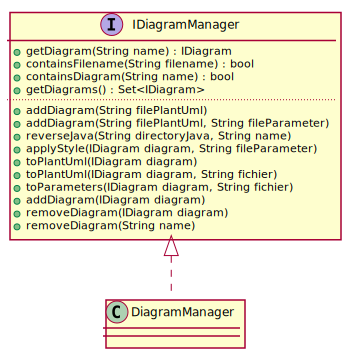
\includegraphics[width=6cm]{Image/manager.png}
	\end{center}
	\newpage
	
	\paragraph{util}
	Ce package contient les différentes classes utilisées par tous les diagrammes. 
	On y retrouve le maximum de code commun comme les \emph{INotes}, les gestionnaires de style et quelques classes abstraites qui peuvent être héritées pour récupérer la mécanique de base des entitées ou des diagrammes. 
	\begin{center}
	  \includegraphics[width=12cm]{Image/util.png}
	\end{center}
	
	\newpage
	\paragraph{Visiteur}
	Il s'agit, dans ce package, de visiteurs qui permettent de lancer sur un diagramme les visiteurs spécialisés pour le typage du diagramme. 
	Cela nous permet de lancer les visiteurs sans connaitre le typage d'un diagramme.
	Les visiteurs permettent de sérialiser un diagramme en fichier de paramètre, de style ou de créer la vue correspondante.
	Chaque diagramme possède son propre package \emph{visiteur} avec les visiteurs propres à exécuter ces fonctionnalités pour le type correspondant.
	\begin{center}
	  \includegraphics[width=10cm]{Image/visiteurGlobaux.png}
	\end{center}
	
          \paragraph{IDiagramClass}
	Cette classe modélise un diagramme de classe en objet. Il est possible d'effectuer tout un tas d'opérations dessus qui vérifient les exigences 
	MOD\_10 MOD\_20 MOD\_30 MOD\_40 MOD\_50 MOD\_60 MOD\_70 MOD\_80 MOD\_90 MOD\_100 MOD\_110 de la STB.
	
	\newpage
	\subparagraph{Les entités}
	Les différentes entitées d'un diagramme de classe sont les énumérations(\emph IEnum), les classes(\emph{IClass}) et les interfaces(\emph{IInterface}). 
	Elles possèdent chacune beaucoup de code commun tout en ayant de grandes disparités de comportements.
	Les énumérations possèdent une liste d'élément.
	Les classes et les interfaces possèdent des méthodes(\emph{IMethod}) ainsi que des attributs(\emph{IAttribute}).
	Les classes associent à chaque méthode et attribut une visibilité (\emph{IVisibility}).
	Les fonctions sont composées d'un nom, d'un type de retour(\emph{IType}) ainsi que d'une liste de variable(\emph{IVariable}).
	Les attributs contient une variable.
	Les variables contiennent un type et un nom.
	Un type possède un nom et, s'il est générique, une liste de type.
  
	\begin{center}
	  \includegraphics[width=12cm]{Image/classExtendUtil.png}
	\end{center}
	\begin{center}
	  \includegraphics[width=14cm]{Image/classe.png}
	\end{center}
	
	\newpage
	\paragraph{Les relations}
	Dans le package relation, on retrouve toutes les relations existantes pour le diagramme de classe. 
	\begin{center}
	  \includegraphics[width=14cm]{Image/classRelation.png}
	\end{center}
	\paragraph{Le visiteur}
	\begin{center}
	  \includegraphics[width=12cm]{Image/classVisiteur.png}
	\end{center}
	
      \subsubsection{IDiagramUseCase}
	Cette classe modélise un diagramme de cas d'utilisation en objet. Il est possible d'effectuer tout un tas d'opérations dessus qui vérifient les exigences 
	MOD\_10 MOD\_20 MOD\_30 MOD\_40 MOD\_50 MOD\_60 MOD\_70 MOD\_80 MOD\_90 MOD\_100 MOD\_110 de la STB.
	
	\newpage
	\paragraph{Les entités}
	\begin{center}
	  Le diagramme d'utilisation possède deux entités : Les acteurs(\emph{Actor}) et les cas d'utilisation (\emph{UseCase}).
	  Chacun ne possède qu'une description et les relations partant d'elle vers une autre entité.
	  \includegraphics[width=16cm]{Image/usecase.png}
	\end{center}
	\paragraph{Les relations}
	Dans le package relation, on retrouve les relations existantes pour le diagramme de cas d'utilisation. 
	\begin{center}
	  \includegraphics[width=10cm]{Image/useCaseRelation.png}
	\end{center}
	\paragraph{Le visiteur}
	\begin{center}
	  \includegraphics[width=12cm]{Image/useCaseVisiteur.png}
	\end{center}
      
    \subsection{IDiagramParser}
	
	\subsubsection{Manager}
	\begin{center}
	  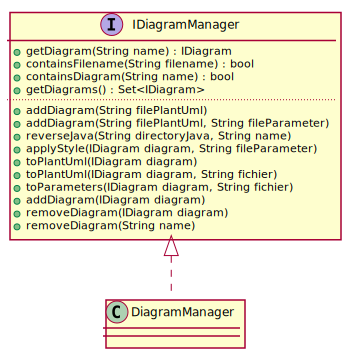
\includegraphics[width=6cm]{Image/manager.png}
	\end{center}
	
	\subsubsection{util}
	\begin{center}
	  \includegraphics[width=12cm]{Image/util.png}
	\end{center}
	\subsubsection{Visiteur}
	\begin{center}
	  \includegraphics[width=10cm]{Image/visiteurGlobaux.png}
	\end{center}
	
    
    \subsection{IDiagramLoader}
   Il s'agit de la classe servant de façade à toutes les fonctionnalités qui nécessitent de parser avec \emph{antlr} un fichier.
   Cette classe permet de créer un diagramme à partir d'un fichier java ou plantuml. 
   Il permet d'appliquer un fichier de style à un diagramme.
   C'est cette classe qui utilise \emph{Dot} pour placer initialiser les diagrammes avec un placement automatique.
   \begin{center}
	  \includegraphics[width=14cm]{Image/parser.png}
	\end{center}
	
   \newpage
   \subsection{filemanager}
   Ce package contient les classes qui gèrent les projets et les différents fichiers contenus. 
   C'est la classe \emph{FileManager} qui sert de modèle pour la partie gauche qui sera définit ensuite.
    \begin{center}
	\includegraphics[width=9cm]{Image/partieGaucheModele.png}
    \end{center}
    
      
   \newpage
  \section{Paquetage ui}
    L'application s'appuie sur la structure JavaFX avec la classe applicative UmlReverseApp qui est composée d'un stage qui en suivant
    la hiérarchie JavaFX nous ammène au BorderPane. Le BorderPane nous servira de base pour les différents éléments de notre application,
    tel qu'une TreeFileManagerView, une MenuBar, un IDiagramEditor et un IDiagramMenu.
    \begin{center}
	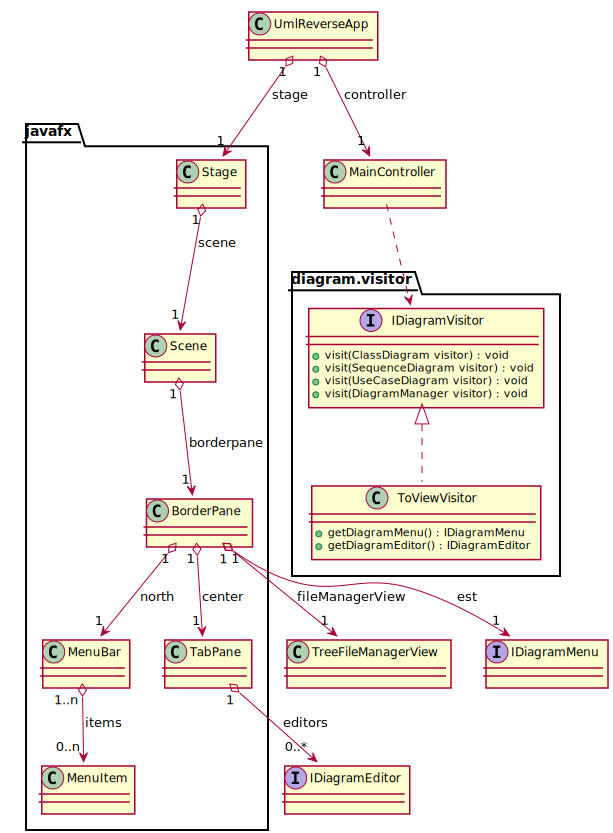
\includegraphics[width=10cm]{Image/Vue.png}
    \end{center}
  
    Ce paquetage contient toutes les classes utilisées pour gérer la vue. Ces classes sont toujours associées à un contrôleur.
    Les vues sont codées en fxml grâce à un logiciel de construction de fxml (SceneBuilder). Chaque contrôleur aura le même nom
    que la vue associée avec le mot ``Controller'' ajouté à la fin.
    ui contient 2 paquetages :
    \begin{itemize}
    \item view : Contient les différentes vues intégrées dans l'application. Le paquetage contient également tous les contrôleurs associés à leur vue.
    \item component : Contient toutes les classes utilisées pour construire les vues. Ce sont leurs composants.
    \end{itemize}
    L'application graphique est l'association de plusieurs vues dans un BorderPane.
    
    \begin{center}
	\includegraphics[width=\textwidth]{Image/maquette.png}
    \end{center}

  \subsection{La partie gauche}
    La partie gauche présente la liste des projets disponibles et des diagrammes qu’ils contiennent, et permet de naviguer entre eux. 
    Cette tâche est accomplie par un modèle qui gère les fichiers, accompagné d’une vue hiérarchique constructible à partir de ce modèle.
    
    \begin{center}
	\includegraphics[width=4cm]{Image/partieGaucheVue.png}
    \end{center}
  \subsection{La partie centrale}
    La partie centrale sert à éditer graphiquement un diagramme. La vue principale de cette partie est codée en fxml: DiagramEditor.fxml. Et
    associé à son contrôleur DiagramEditorController.java.\\
    
    \textbf{\underline{Explication}}: Toutes les classes qui finissent par Graphic sont des réprésentations graphiques des élements du modèle. Elles contiennent
    des écouteurs de souris sur elles mêmes pour pouvoir permettre aux utilisateurs de les modifier ce qui modifiera le modèle directement.
    La modification du modèle modifie obligatoirement la vue du diagramme (les éléments graphiques donc) grâce à des écouteurs sur le modèle.
    
    \subsubsection{Editeur de diagramme}
	La partie MVC a été volontairement omise pour éviter de surcharger le diagramme de classe. Elle sera 
	par contre implémenté dans les parties prévues.\\
	Dans les diagrammes ci contre les contrôleurs controleront les actions de IDiagramEditor.\\
	Nous appelons les éditeur de diagrammes des IDiagramEditor. Nous en avons 2 différents, un pour chaque type de diagramme à éditer.
	\paragraph{Paquetages}
	  \subparagraph{Les entités}
	  \begin{center}
	      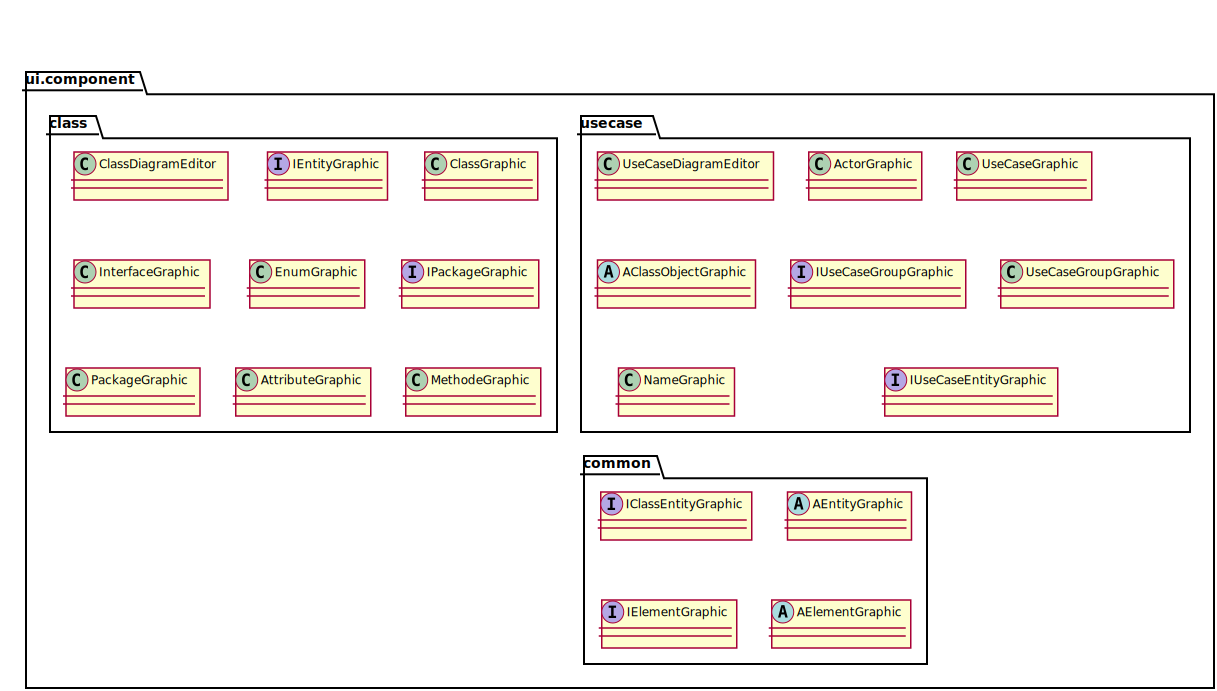
\includegraphics[width=\textwidth]{Image/DiagramEditor_EntityPackage.png}
	  \end{center}
	  \subparagraph{Les relations}
	  \begin{center}
	      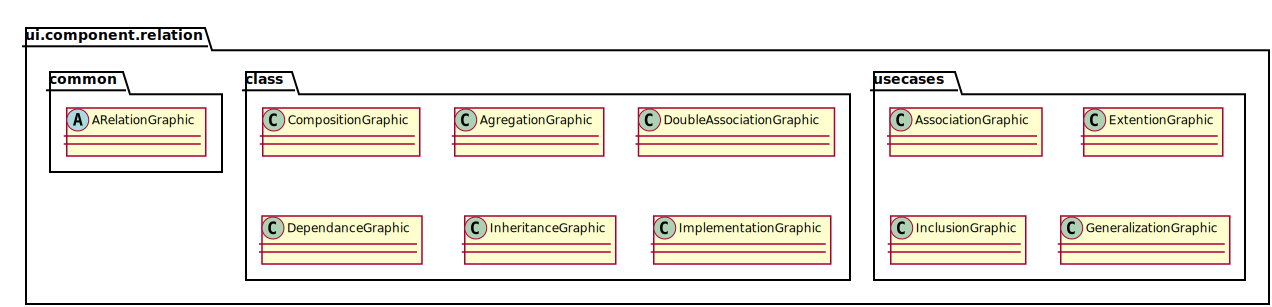
\includegraphics[width=\textwidth]{Image/DiagramEditor_RelationPackage.png}
	  \end{center}
	  
	  \newpage
	\paragraph{Diagramme de classe}
	\begin{center}
	    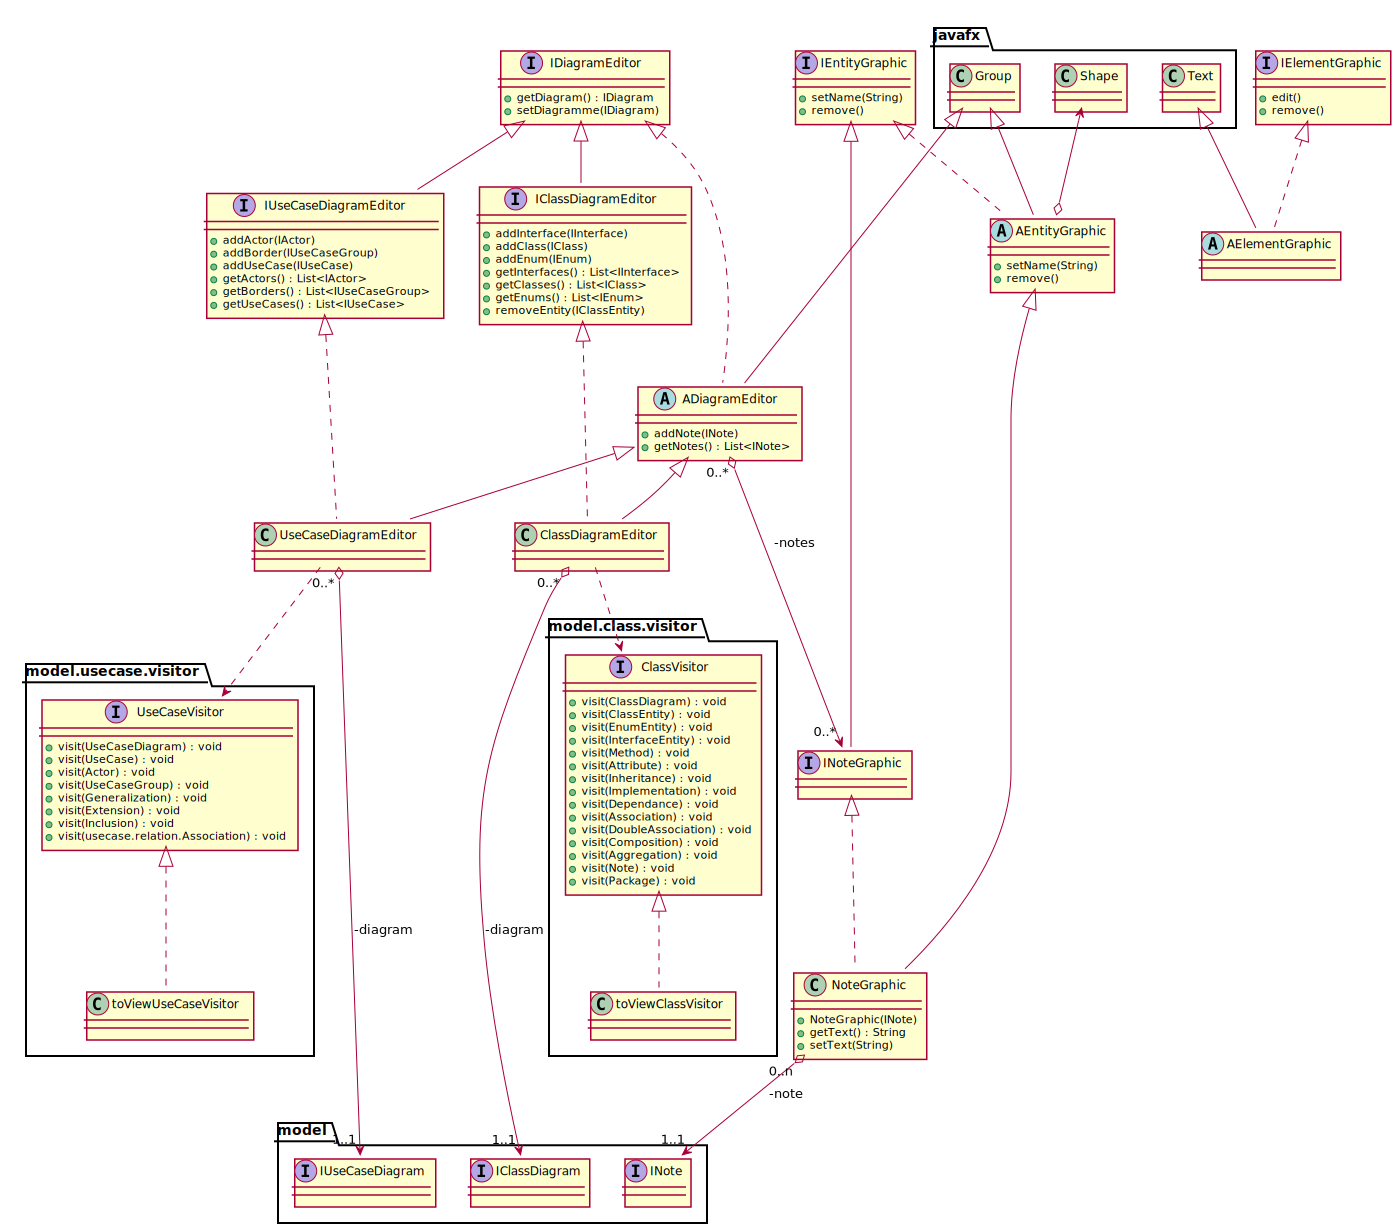
\includegraphics[width=\textwidth]{Image/DiagramEditorGeneral.png}
	\end{center}
	Dans ce diagramme il se trouve les deux DiagramEditor prévus pour ce produit avec les classes qu'elles ont en commun.
	Les visiteurs de ce diagramme servent à dessiner la vue.
	
	\newpage
    \subsubsection{Editeur de diagramme de classe}
	 \paragraph{Gestion des entités}
	  \begin{center}
	      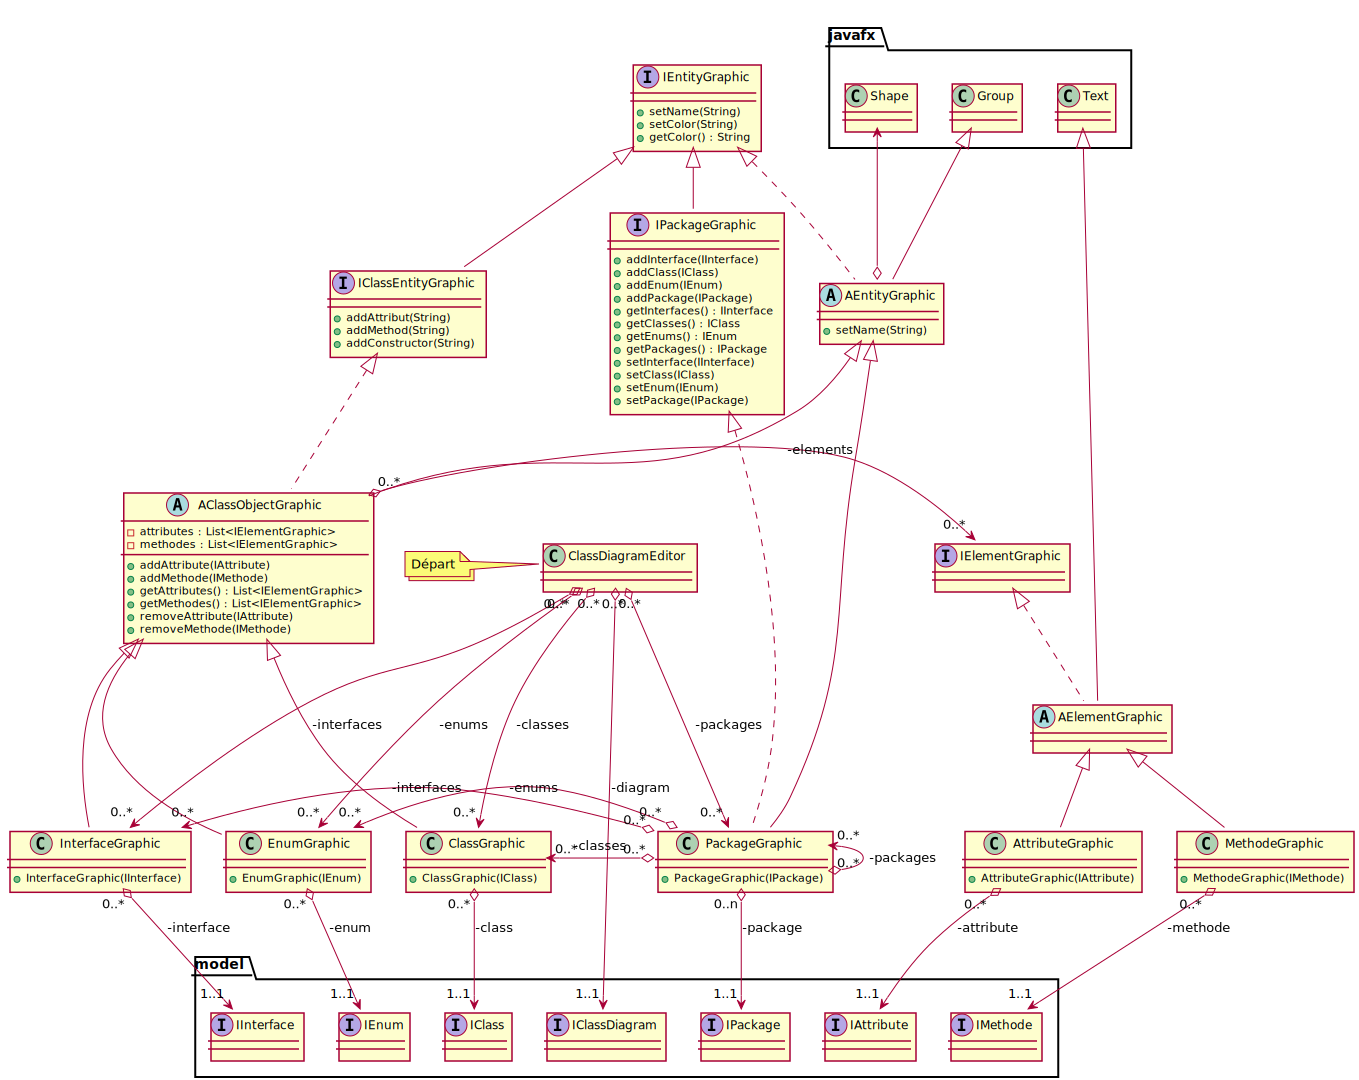
\includegraphics[width=\textwidth]{Image/ClassDiagramEditor.png}
	  \end{center}
	  
	 \paragraph{Gestion des relations}
	  \begin{center}
	      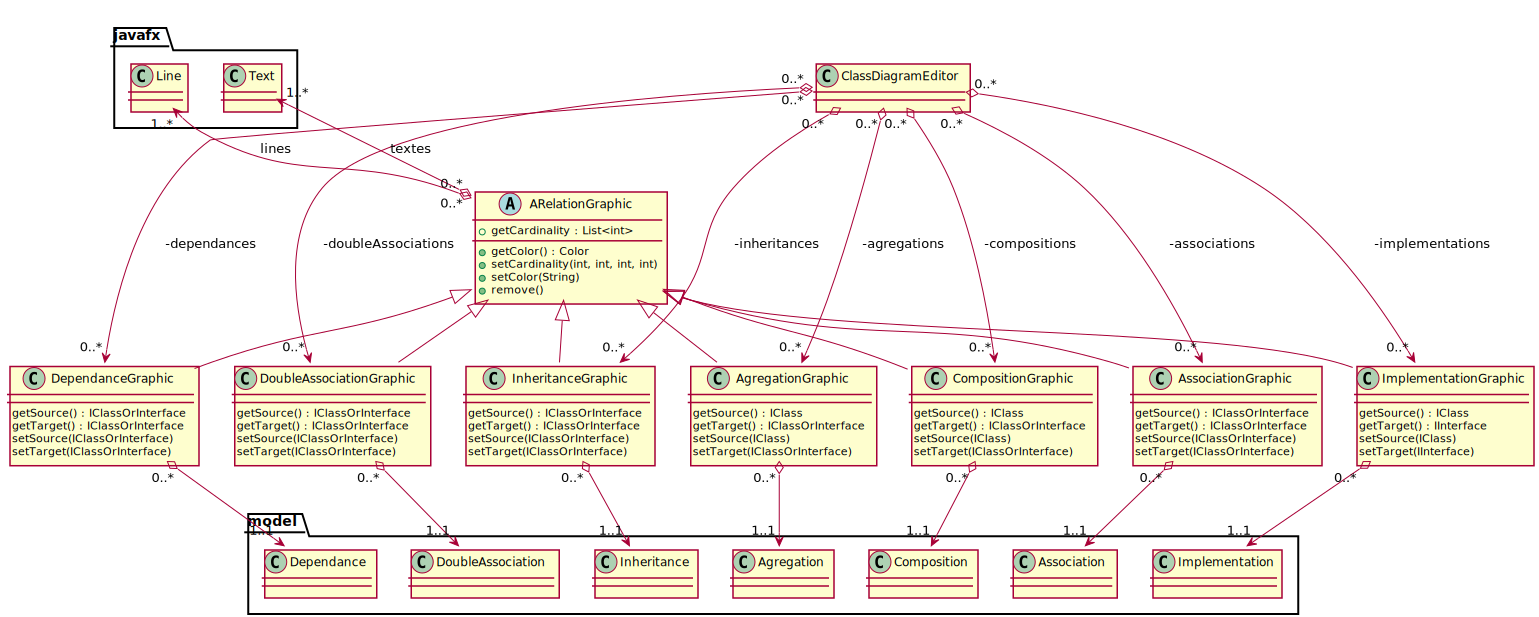
\includegraphics[width=\textwidth]{Image/ClassDiagramEditorRelation.png}
	  \end{center}
	  
	  \newpage
   \subsubsection{Editeur de diagramme de cas d'utilisation}
	 \paragraph{Gestion des entités}
	  \begin{center}
	      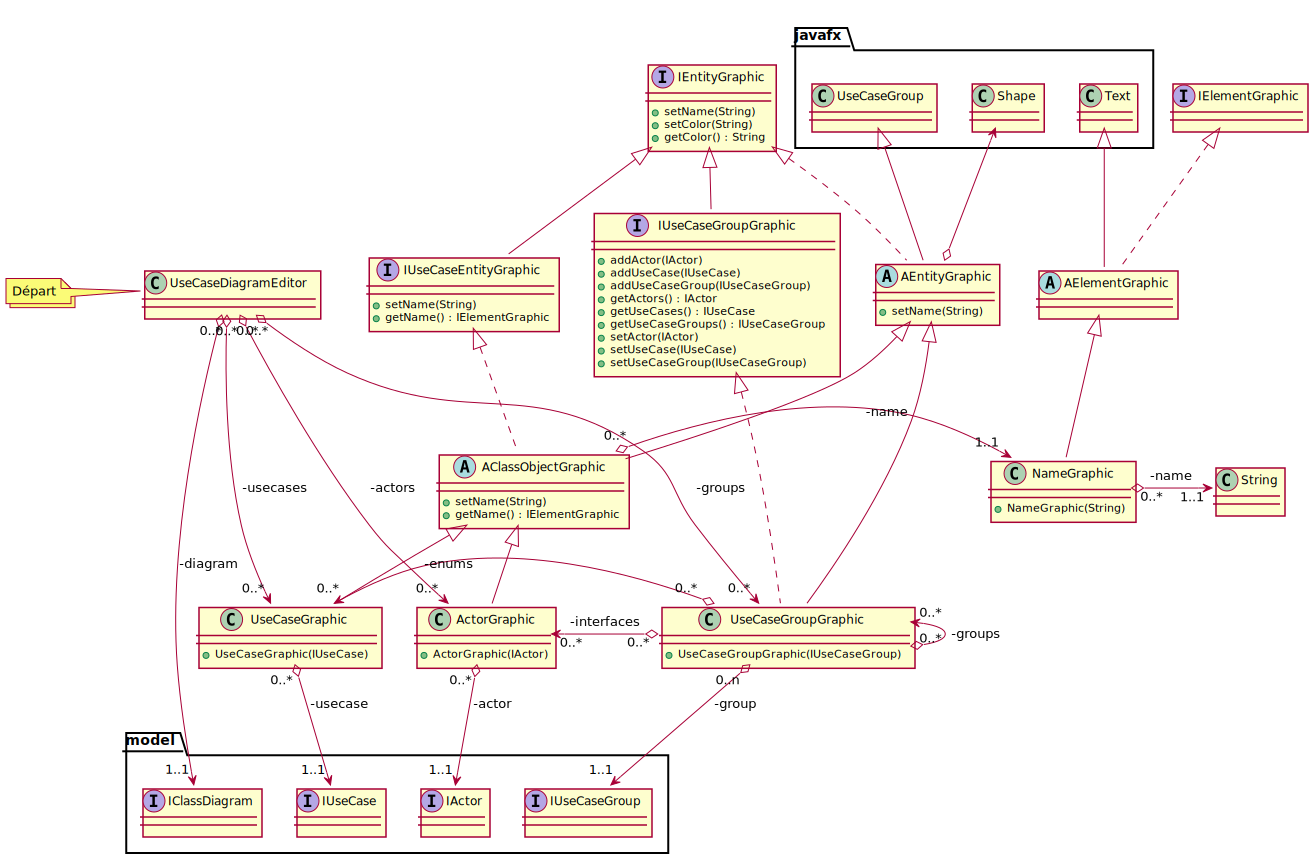
\includegraphics[width=\textwidth]{Image/UseCaseDiagramEditor.png}
	  \end{center}
	  
	 \paragraph{Gestion des relations}
	  \begin{center}
	      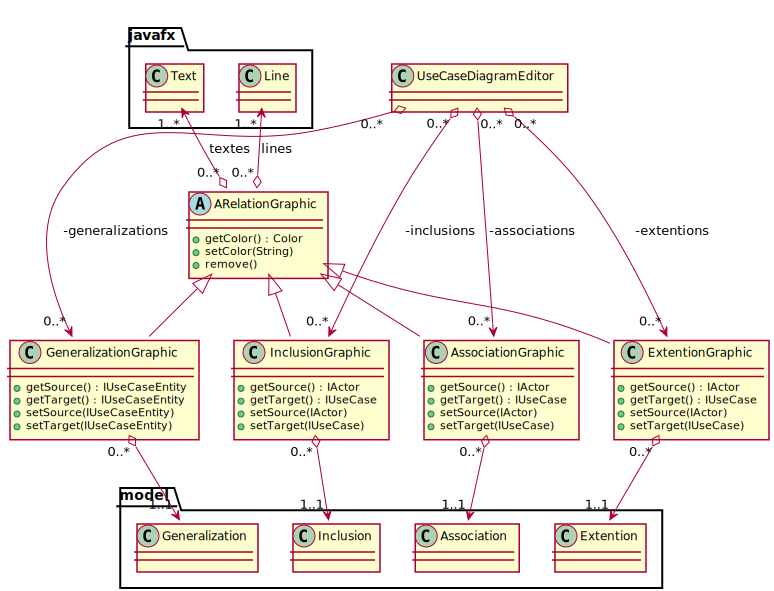
\includegraphics[width=12cm]{Image/UseCaseDiagramEditorRelation.png}
	  \end{center}
   
    \subsubsection{Explications}
	\begin{center}
	  \includegraphics[width=\textwidth]{Image/demonstration.png}
	\end{center}
      
  \subsection{La partie droite}
    \subsubsection{Déroulement}
      Quand un utilisateur séléctionne un diagramme l'action fait appel au contrôleur qui va passer par l'interface IDiagram du modèle et le visiteur 
      permet de déterminer le type de diagramme selectionné.
      L'interface IDiagramMenu nous permet d'ajouter des entités et des relations dans un diagramme grâce au contrôleur qui gère les actions.
       
    \subsubsection{Diagramme de classe} 
          \begin{center}
	     \includegraphics[width=15cm]{Image/DiagramGenrDroite.png}
          \end{center}
          
\section{Paquetage main}
    Contient la classe qui lance l'application. C'est le point d'entrée. Il charge les différentes vues du paquetage ui.view en les rassemblant toutes dans un BorderPanel.
    
\section{Diagramme de Séquence}
  \subsection{Ouverture de l'application}
  \begin{center}
	     \includegraphics[width=14cm]{Image/Diag_Seq_Open.png}
   \end{center}
    
   \subsection{Chargement d'un diagramme dans la vue}
   \begin{center}
	     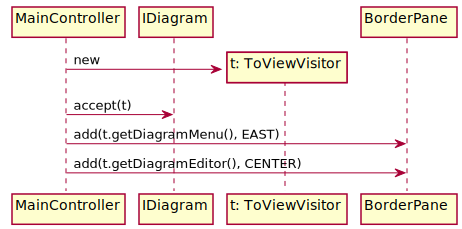
\includegraphics[width=8cm]{Image/uiupdate.png}
   \end{center}
   
   \subsection{Chargement d'un fichier java}
    \begin{center}
	     \includegraphics[width=10cm]{Image/Charge_File_Java.png}
    \end{center}
  
\section{Extensibilité}
  L'architecture a été pensé de façon à vérifier l'exigence EXF\_70 (code modulaire, ajout de nouvelles fonctionnalités possible dans le code).
  \paragraph{Modèle}
    Le modèle a été pensé à facilement ajouter de nouveau type de diagramme. Pour ce faire le gestionnaire de diagramme ne se soucis pas du type de diagramme.
    La plupart des actions demandées sur un diagramme de manière extérieur au modèle se font par le biais des visiteurs. Pour ajouter un nouveau
    type de diagramme il suffit de créer une nouvelle classe qui implémente IDiagram et de mettre à jour les visiteurs globaux.
  \paragraph{Partie gauche de l'application}
    Les différentes classes créées peuvent être héritées afin d'étendre leurs fonctionnalitées ainsi que d'ajouter de nouveaux types de diagramme. 
    L'architecture des dossiers d'un projet a été pensée afin que l'ajout de nouveau type de fichier pour la sauvegarde des diagrammes
    soit simple sans rendre les projets de cette version obsolète.
  \paragraph{IDiagramEditor}
    Tout d'abord, l'ajout de nouveau type de diagramme a été pensé de façon à être possible et facile à implémenter. 
    Pour se faire, il suffit d'ajouter dans le IDiagramEditor une 
    nouvelle classe XXXDiagramEditor. Cette nouvelle classe peut hériter ADiagramEditor si le nouveau type de diagramme peut posséder des notes.
    L'implémentation de celle ci sera déjà implémentée.
    Les classes présentes dans le paquetage view.component.common sont des classes qui peuvent être utilisées dans n'importe qu'elle type de diagramme. Ce
    sont généralement des classes abstraites qui font une partie du travail. Ce qui évite de tous refaire à chaque fois.
    
  \paragraph{IDiagramMenu}
    Cette partie peut aussi facilement ajouter des nouveaux types de diagrammes. Il suffit de rajouter un nouveau type de menu et d'implémenter la bonne interface.

    \newpage
\section{Annexe}
  \subsection{Modèle du diagramme de séquence}
      Les diagrammes suivants ont été pensés au cas où nous arrivions à finir le projet avec de l'avance.
    \begin{center}
	  \includegraphics[width=12cm]{Image/sequence.png}
	\end{center}
	\begin{center}
	  \includegraphics[width=14cm]{Image/sequenceBlock.png}
	\end{center}
	\begin{center}
	  \includegraphics[width=12cm]{Image/sequenceMessageBlock.png}
	\end{center}
	\begin{center}
	  \includegraphics[width=12cm]{Image/sequenceMessageInline.png}
	\end{center}
	\begin{center}
	  \includegraphics[width=12cm]{Image/sequenceVisiteur.png}
	\end{center}



\begin{comment}
  \subsection{model}
  Ce package contient l'intégralité du modèle. Il contient tous les packages et classes pour le travail métier.
  \subsubsection{util}
  Le code commun à tous les diagrammes
  \begin{center}
      \includegraphics[width=\textwidth]{Image/util2.png}
  \end{center}
  \begin{landscape}
      \includegraphics[height=12cm]{Image/utilDiagramme.png}
  \end{landscape}
  Ce package contient l'intégralité du code commun à chaque diagramme. 
  C'est aussi ici qu'on trouve la définition des boîtes de style.
  \subsubsection{visitor}
  Les visiteurs permettent l'ajout d'opérations homogènes à des entités d'un modèle sans couplage.
  \begin{center}
      \includegraphics[width=\textwidth]{Image/visitor.png}
  \end{center}
  Ce package contient les visiteurs des diagrammes.
  \subsubsection{classDiagram}
  \begin{center}
      \includegraphics[width=\textwidth]{Image/classDiagramUp.png}
  \end{center}
  \begin{center}
      \includegraphics[width=12cm]{Image/classDiagramBottom.png}
  \end{center}
  Ce package contient le code pour stocker un diagramme de classe extrait à partir d'un fichier java. 
  A fortiori, il gère tout diagramme de classe en plantUml représentant un diagramme de classe valide en UML2.
  \subsubsection{sequenceDiagram}
  \begin{center}
      \includegraphics[width=\textwidth]{Image/SequenceDiag.png}
  \end{center}
  \begin{center}
      \includegraphics[width=\textwidth]{Image/SeqBlocksDiag.png}
  \end{center}
  Ce package contient le code pour stocker un diagramme de séquence. 
  Il gère tout diagramme de séquence en plantUml représentant un diagramme de séquence valide en UML2.
  \subsubsection{useCaseDiagram}
  \begin{center}
      \includegraphics[width=\textwidth]{Image/UseCaseDiag.png}
  \end{center}
  Ce package contient le code pour stocker un diagramme de cas d'utilisation. 
  Il gère tout diagramme de cas d'utilisation en plantUml représentant un diagramme de séquence valide en UML2.
  \subsubsection{parser}
   Les imports
  \begin{center}
      \includegraphics[width=\textwidth]{Image/parser.png}
  \end{center}
  Ce package contient les différents parsers qui seront utilisées pour extraire le style, le plantUml et le java.

  \subsection{ui}
  Ce package contient l'intégralité de la vue et des contrôleurs.
  \subsubsection{view}
  C'est dans ce package que se situe les différentes vues utilisées par l'application.
  \subsubsection{controllers}
  Ce package contient toutes les classes permettant la communication entre la vue et le modèle.
  \subsubsection{components}
  Les différents composants de l'ihm
  \begin{center}
      \includegraphics[width=\textwidth]{Image/Component.png}
  \end{center}
  Ce package contient les composants qui seront utilisées par la vue.
  
\section{}
\end{comment}

\end{document}
